\documentclass[
  utf8,%     More capable input encoding than latin-1.
  parskip,%  For vertical whitespace between paragraphs.  This comes down to more than just using parskip.sty, so it's better to use this class option.
  % S5MP % If you intend to really use margin paragraphs (not recommended!).
%  crop,%     Produce output with crop marks and paper size A4.  Liu-Tryck should like this.  Automatically adds information, including the physical page number, at the top of each page.
       %     Add option 'noInfo' to suppress the info at the top of each page when using option 'crop'.
  % Font options: 'kp' (default), 'times', 'lm'.  The KpFonts (loaded using 'kp'), is the most complete font among the provided options.  Among other, it supports slanted small caps.  See rtthesis.cls for more details regarding the font options.
  largesmallcaps,intlimits,widermath,% Good options to KpFonts.
  sharecounter,nobreak,definition=marks,%  See comments in the results chapter of this document for more information on these options!
  %numbers, % If you want to cite references by numbers, use this option.
  noparts% Use option 'noparts' if you do not make use of part divisions.
]{rtthesis}

\usepackage{mythesis}


\begin{document}
\selectlanguage{english}
\makeFrontPage
\frontmatter
\maketitle
\makeLibraryPage{Det här som vi har hållit på med är jätteviktigt faktiskt och det vi gjort blev bara sååå bra.  Kanske inte helt otippat, men det glass är sååå gott!

Förresten har vi blivit bäst på att skriva rapporter, så nu ska ska vi inte gå in närmare på några detaljer såhär i sammanfattningen.
}

\begin{abstract}[swedish]
  Det här som vi har hållit på med är jätteviktigt faktiskt och det vi gjort blev bara sååå bra.  Kanske inte helt otippat, men det glass är sååå gott!

Förresten har vi blivit bäst på att skriva rapporter, så nu ska ska vi inte gå in närmare på några detaljer såhär i sammanfattningen.

\end{abstract}
\begin{abstract}[english]
  If your thesis is written in English, the primary abstract would go here while the Swedish abstract would be optional.

\end{abstract}
\begin{acknowledgments}
  Vi tycker alla har varit så himla goa hela den här långa och tuffa tiden i våra liv.

  \addvspace{1em}
  \begin{flushright}
    \textit{%
      Linköping, Januari 2020\\
      N N och M M%
    }
  \end{flushright}
\end{acknowledgments}

\tableofcontents
\begin{notation}% Passing the option "old" to the notation environment will redefine the notationtabular environment so that it produces an old style LaTeX tabular instead of a ctable.sty style tabular.
  \centering

  \begin{notationtabular}{Några mängder}{Notation}{Betydelse}
    $\naturals$ & Mängden av naturliga tal \\
    $\reals$ & Mängden av reella tal \\
    $\complexes$ & Mängden av komplexa tal \\
  \end{notationtabular}

  \begin{notationtabular}{Förkortningar}{Förkortning}{Betydelse}
    \abbrARMA\index{ARMA@\abbrARMA!abbreviation} & Auto-regressive moving average \\
    \abbrPID\index{PID@\abbrPID!abbreviation} & Proportional, integral, differential (regulator) \\
  \end{notationtabular}
\end{notation}


\mainmatter
\chapter{Introduction}
\label{sec:introduction}

Text\dots

\section{Some \LaTeX\ resources}
\label{sec:section1}

A great starting point when you are new to \LaTeX\ is to read
\cite{oetikerPHS:2004}.

There are many interesting things about \LaTeX\ found in the standard
references by Lamport \cite{lamport:1994} and Gossens et al.\
\cite{companion:2004}. These describe most everything one needs to
know about creating documents with \LaTeXe.  Gossens et al.\ has also
written a book dealing with graphics in \LaTeX, mostly Post-Script
based, \cite{companionG:1997}. Of course there exists many other good
references to \LaTeX\ out there too.

\begin{example}[An example of an example]
  In this example please note that there is a substantional difference
  between \cite{companion:2004} and the first edition of the book
  \cite{companion:1994}.
\end{example}

% Local Variables:
% TeX-master: "main.tex"
% End:

\chapter{System overview}
\label{sec:System overview}
The system for detection of barcodes is basically divided in two parts. The data consist of a big amount of images which contain 1D- and 2D-codes. Each image has a corresponding ground truth where the parts of the image containing codes has been labeled as "true" and the rest as "false". The first part of the system involves the training using machine learning which produces a classifier. It consists of the following steps.

\begin{itemize}
	\item Preprocessing of images.
	\item Divide images and ground truth into tiles.
	\item Calculate features for each tile.
	\item Use machine learning to train the dataset.
\end{itemize}

The objective of the second part of the system is to predict unlabeled data in real time. This is done with the trained classifiers and a cascade. It involves the following steps:

\begin{itemize}
	\item Preprocessing of image.
	\item In each step of the cascade calculate some specific features.
	\item Use the corresponding classifier for each feature to reduce the amount of data between each step in the cascade.
	\item Postprocessing of the output.
\end{itemize}
An overview of the system can be seen in \ref{system}.

%Flow chart
\begin{figure}[H]
\centering
\tikzstyle{largeblock} = [rectangle, draw, fill=blue!20, 
    text width=10em, text centered, rounded corners, minimum height=5em]
\tikzstyle{block} = [rectangle, draw, fill=blue!20, 
    text width=5em, text centered, rounded corners, minimum height=4em]
\tikzstyle{line} = [draw, -latex']
\tikzstyle{cloud} = [draw, ellipse,fill=red!20, node distance=3cm,
    minimum height=2em]
    
\begin{tikzpicture}[node distance = 2.5cm, auto]
    % Place nodes
    \node [cloud] (training) {labeled training data};
    \node [largeblock, below of=training] (machine) {training using machine learning};
    \node [block, below of=machine] (classifier) {classifier};
    \node [cloud, right of=training, node distance=4cm] (test) {test data};
    \node [block, below of=test, node distance=5cm] (cascade) {cascade};
    \node [block, below of=cascade] (prediction) {prediction};
    
    
    % Draw edges
    \path [line] (training) -- (machine);
    \path [line] (machine) -- (classifier);
    \path [line] (classifier) -- (cascade);
    \path [line] (test) -- (cascade);
    \path [line] (cascade) -- (prediction);

\end{tikzpicture}
\caption{Overview of the system}
\label{system}
\end{figure}




% Local Variables:
% TeX-master: "main.tex"
% End:

\chapter{Data processing}
\label{sec:Data processing}

\section{The dataset}
\label{The dataset}
The dataset consists of a big amount of gray scale images containing 1D- and 2D-codes of different sizes and orientation. For each image the corresponding ground truth are also available. The images are first of all divided into one training dataset and one testing dataset. Each image are then divided into tiles of the same size. 
\begin{center}
	$x = [x_1,...,x_N]$
\end{center}
With corresponding ground truth:
\begin{center}
	$y = [y_1,...,y_N]$
\end{center}
The tiles can either overlap each other or just lay next to each other. For each tile a number of different features will be calculated, i.e. each tile consists of a feature vector:
\begin{center}
\begin{math}
	x_i =  
	\begin{pmatrix}
		 f_1 \\ \vdots \\ f_M
	\end{pmatrix}
\end{math}
\end{center}  
The features are in some way based on the pixel values in the tile.

During testing each data will get a prediction. These can have four different states based on the relation between the prediction and the ground truth:
\begin{itemize}
	\item true true
	\item false true
	\item true false
	\item false false
\end{itemize}

\section{Preprocessing}
\label{Preprocessing}
Some of the features used in the system gives better result with some preprocessing. The reason for this is that the codes in some of the images have less contrast than others. Here a Laplace filter is applied to the images to make them a bit sharper. However some of the features gives better result without any preprocessing, therefore the filtered images are only used for calculation of some of the features.

\section{Postprocessing}
\label{Postprocessing}
At the end of the cascade when all the test data have been predicted there are some postprocessing before obtaining the final result. The reason for this is to remove some possible true false classifications. The false classifications are often distinctive since the true true classifications usually lay in clusters. Here a filter is applied which removes isolated true classifications. After that some morphological operations are done fill some possible holes in the areas where the codes are.
% Local Variables:
% TeX-master: "main.tex"
% End:

\chapter{Machine learning methods}
\label{sec:Machine learning methods}

\section{Discrete AdaBoost}
\label{sec:Discret AdaBoost}
For detection of barecodes the machine learning method discrete AdaBoost has been used which is described in \citep{Friedman:2000}. The algorithm is described in \ref{AdaBoost}. The basic idea is to train a number of weak classifiers which during the testing will be combined to a strong classifier. To each data in the training dataset there are corresponding weights which are equal for all data at the beginning. The weak classifiers are trained sequentially and after each step the weights are adjusted depending if they were correctly or incorrectly classified.

\begin{figure} [H]
\line(1,0){250} \newline
Given: $(x_1,y_1),...,(x_m,y_m), \text{where } x_i\in X, y_i \in [-1,+1]$. \newline
$\text{Initialize: } D_1(i)=1/m \text{for } i=1,...,m.$ \newline \newline
$\text{For } t=1,...,T:$
\begin{itemize}
\item $\text{Train weak learner using distribution } D_t.$
\item $\text{Get weak classifier } h_t : X \to {-1,+1}$.
\item \text{Aim: select with low weighted error:}
\begin{center} 

	$\epsilon_t = \sum_{i=1}^{m} D_t(i)I(y_i ! h_t(x_i))$ \newline
	$\text{where I is the split function}$ \newline
\end{center}
\item Chose $ \alpha_t = \frac{1}{2}(\frac{1-\epsilon_t}{\epsilon_t})$
\item Update, for $t = 1,...,m:$
\begin{center} 

	$D_{t+1}(i) = \frac{D_t(i)exp(-\alpha_ty_ih_t(x_i)}{Z_t}$ \newline
	Where $Z_t$ is a normalization factor. \newline
\end{center}
\end{itemize}
Final strong classifier
\begin{center}
	$ H(x) = sign(\sum_{t=1}^{T} {\alpha_th_t(x)}-\phi)$
\end{center}
\line(1,0){250}
\caption{Algorithm for discrete AdaBoost}
\label{AdaBoost}
\end{figure}


The split functions may consist of a number of different parameters. The most basic function, which has been used here, only has one parameter, a threshold. The function search for a threshold in one dimension at a time and choose the one whish best separates the data. 
% Local Variables:
% TeX-master: "main.tex"
% End:

\chapter{Features}
\label{sec:Features}

\section{Features used to detect barcodes}
\label{sec:Features used to detect barcodes}
Several different features has been tried out but many of them have not given any satisfying result. Here are the features that have shown  best result.
\subsection{Standard deviation}
\label{sec:Standard deviation}
One good method to exclude tiles that don't contain any code is to compute the standard deviation of each tile. Tiles which contain code will have a high standard deviation; hence all data with standard deviation under a certain threshold can be discarded. This fast method to reduce the amount of data before applying other more complicated features. 

\subsection{Structure tensor}
\label{sec:Structure tensor}
The structure tensor is an effective way to detect 1D-codes and to distinguish between 1D- and 2D-codes. The structure tensor for a tile is produced by first computing the gradients, this can be done by convolving the tile with a sobel filter. The structure tensor is then calculated in the following way:
\begin{center}
\begin{math}
	T = \begin{pmatrix}
			(I_{x})^2 & I_{x}I_{y} \\ I_{x}I_{y} & (I_{y})^2
		\end{pmatrix}
\end{math}
\end{center}
The structure tensor can be used in several ways to estimate the structure inside the tile. Areas that contain 1D-codes will have a one dimensional structure, i.e. the gradient in this area will only vary in one direction. On the other hand, areas that contain 2D-codes the variation will be fairly equal in both directions. The amount of variation of the gradient is measured by studying the eigenvalues of the structure tensor. The following feature is calculated for each tile:
\begin{center}
\begin{math}
f = \frac{(\lambda_1 - \lambda_2)^2}{\lambda_1^2+\lambda_2^2}
\end{math}
\end{center}
This feature is a measure of how likely the tile contains 1D-codes.

\subsection{FAST corner detection}
\label{sec:FAST corner detection}
FAST (Features from Accelerated Segment Test) is described in \citep{Rosten:2006} and \citep{Rosten:2005}. This is a method to detect corners in images, which is a good way to distinguish between 1D- and 2D-codes. For a pixel \textit{p} with intensity \textit{I}, consider a circle of 16 pixel and a threshold \textit{t}. The pixel is considered to be a corner if there exist a set of n contiguous pixels in the circle which are all brighter than \textit{I+t} or darker than \textit{I-t}. The algorithm is described in \ref{FAST}.

\begin{figure}[H]
\centering
	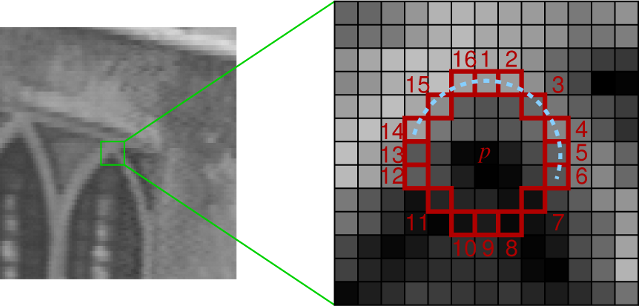
\includegraphics[scale=0.5]{FAST}
	\caption{Image describing FAST corner detection}
	\label{FAST}
\end{figure}

\subsection{Distance map}
\label{sec:Distance map}
A method for barcode detections using a distance map is described in \citep{Bodnar}. The objective of this method is to first calculate the edges in the image by using the canny edge detection algorithm. After that a distance transform is used which in each pixel calculates the closest distance to an edge. There after the mean and standard deviation for the distance map are calculated which are then used as features. The distance map has in this system been used only for detection of 1D-codes.
 
\subsection{Local binary pattern}
\label{sec:Local binary pattern}
Local binary pattern, which is described in \citep{Pietikainen:2010}, is a method that can be used for detection of 2D-codes. The basic idea is to compute a binary code for every pixel, based on the difference of the intensity between the pixel and the surrounding pixels, illustrated in \ref{LBP}. The binary code will then be transformed to a decimal scalar value. If a 3x3 neighbourhood is used there will be 256 different possible values. For each block a histogram will be calculated for all these values. Every bin in the histogram will then be used as a feature. If there is a bin for every possible value, there will be 256 features.

\begin{figure}[H]
\centering
	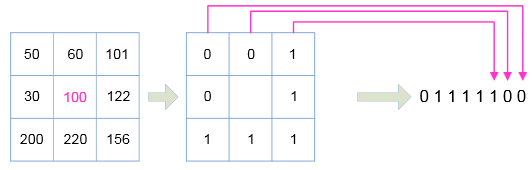
\includegraphics[scale=0.5]{LBP}
	\caption{Image describing local binary pattern}
	\label{LBP}
\end{figure}

\section{Features used for OCR}
\label{sec:Features used for OCR}
Here are the features that have been used for character detection.

\subsection{Two-rectangle features}
\label{sec:Two-rectangle features}
The two-rectangle features are based on the same idea as the Haar-features presented in \citep{Viola:2010}. This method was used in an earlier project regarding OCR at SICKIVP and showed a rather good result. For that reason it has been tried out in this project as well. The main concept is to use a large number of filters in different sizes consisting of two areas. The result from the filters will then be the difference of the sum of the pixel values between the two areas. There are 17 different filters illustrated in \ref{Two-rectangle} each in 64 different sizes. The sizes are in the range:
\begin{center}
	12x12, 12x16, 16x12, 16x16, 16x20, 20x16, 20x20......40x40
\end{center}
The filters can also have different positions which depends on the size of the tile that is used. For example if the tile has the size 120x120 a filter with the size 12x12 can have totally 100 positions without overlapping each other. For a tile with the size 120x120 there will in total be 28578 different features.  
\begin{figure}[H]
\centering
	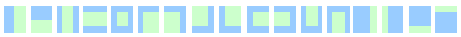
\includegraphics[scale=1]{rectfeatures}
	\caption{Image describing different types of two rectangle features}
	\label{Two-rectangle}
\end{figure}

To make the calculation of the rectangle features faster a s.k. integral image is used. This is a method presented in \citep{Viola:2010} for calculation of Haar-features. An integral image has the same size as the original image. The value for a pixel in the integral image is the sum of all the pixels above and to the left in the original image. If the $i(x,y)$ is the original image the integral image $ii(x,y)$ will be the following.

\begin{center}
	$ii(x,y) = \sum_{x' <= x, y' <= y} i(x',y')$
\end{center}

\subsection{Random point pairs features}
\label{sec:Random point pairs features}
One type of feature that has been tried out for OCR is a method presented in \citep{Nenad}. The idea is to compare a large amount of point pairs in a tile. The point pairs are randomly chosen but with some constraint. The first point in each pair is chosen from the central part of the tile and the the second point is chosen from the whole tile. There is also a constraint of the distance between the points in each pair. The reason for this is that the character should be somewhat centralized in the tile. If both points are at the edge of the image or if they are too close to each other there will likely be less information to gain. The same point pairs are used for every tile both during training and testing. For each tile the corresponding pixel values are compared in the following way:
 \begin{center}
\[ f_i = \left\{ 
   \begin{array}{l l l}
     1 & \quad I(p_1)<I(p_2)\\
     -1 & \quad I(p_1)>I(p_2)\\
     0 & \quad \text{otherwise}
   \end{array} \right.\]
 \end{center}
Each point pair will then correspond to a feature which can have one of three different values. 
\begin{figure}[H]
\centering
	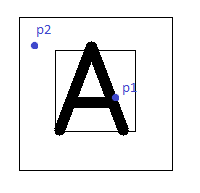
\includegraphics[scale=1]{PointPairs}
	\caption{Image describing two point pairs in a tile}
	\label{PointPairs}
\end{figure}


% Local Variables:
% TeX-master: "main.tex"
% End:

\chapter{Cascade}
\label{sec:Cascade}
\chapter{Evaluation}
\label{sec:Evaluation}
Here is a compilation of the evaluation that has been made for different methods for detections of barcodes. First some results from the different features are evaluated individually regarding their accuracy. Then the accuracy and the speed of the whole system is evaluated.

To get a measure of the accuracy of the system the number of true detections and the number of false detections are calculated and plotted. There are a lot of parameters and variation of the preprocessing of the tiles that will affect the result:

 \begin{itemize}
 	\item Size of the tiles
 	\item Use of overlapping tiles or not
 	\item Use of down sampling
 	\item $\varphi$ from the algorithm in figure \ref{AdaBoost}
 	\item Use of Laplace filtering 
 \end{itemize}

In the evaluation 265 images has been used containing 1D-codes and 2D-codes. Of them 100 has been used for training and 165 for testing.

\section{Calculation of ground truth}
\label{sec:Calculation of ground truth}
One of the problems that can occur with too big tiles and when if the down sampling is too high is that the ground truth is not calculated correctly. Since 70\% of the tile has to be inside the code area there is a chance some codes will be missed out entirely. This is primarily the case for the 1D-codes since some of them are very thin. There are not really any good way to evaluate this except pick out some difficult images and look at the result. If the the tile size is too big to detect some of the codes one solution is to make them overlap with each outer. 

In the table below some tile sizes have been tried out with different down sampling. The values written in the table is how much overlap of the tiles which is necessary to achieve an acceptable result. The places in the table which is empty are cases when it's not possible to get a good result.

\begin{table}[H]
\begin{center}
     \begin{tabular}{ | l | l | l | l | l | p{5cm} |}
     \hline
     tile size & no down sample & down sample 2 & down sample 3 & down sample 4 \\ \hline
   	 24x24 & 1 & 1-2 & 3 & 	\\ \hline
     32x32 & 1 & 2-3 &   & 	\\ \hline
     48x48 & 2 &     &   &  \\ \hline
     64x64 & 3 &     &   &	\\ \hline
     \end{tabular}
\end{center}
\caption{Necessary overlap of the tiles to calculate ground truth}
\end{table}

\section{Evaluation of features}
\label{sec:Evaluation of features}
Here is an evaluation of each feature that are used in the cascade. The objective is to keep as many true tiles as possible in each step of the cascade and in the same time reduce the amount of date as much as possible. In this evaluation the objective has been to preserve at least 98\% of the true tiles in each step. Here different tile sizes and different amount of down sampling have been tried and best value of $\varphi$ has been calculated to preserve 98\% of the true tiles and as few false tiles as possible. Here only cases which gave a good result in the evaluation of the ground truth above are tested. 

\subsection{Standard deviation}
When using standard deviation the images have been preprocessed with Laplace filtering and no overlapping tiles. It has been trained on both 1D- and 2D-codes. 

\begin{table}[H]
\begin{center}
     \begin{tabular}{ | l | l | l | l | l |}
     \hline
     tile size & no down sample & down sample 2 & down sample 3 \\ \hline
   	 24x24 & 4 & 4 & 4 			\\ \hline
     32x32 & 4 & 4  & 			\\ \hline
     48x48 & 3 &     &  		\\ \hline
     64x64 & 3 &     &			\\ \hline
     \end{tabular}
\end{center}
\caption{Lowest value of $\varphi$ that keeps at least 98\% of the true tiles when using standard deviation}
\end{table}

\begin{table}[H]
\begin{center}
     \begin{tabular}{ | l | l | l | l | l |}
     \hline
     tile size & no down sample & down sample 2 & down sample 3 \\ \hline
   	 24x24 & 280 & 12.23 & 33.6 	\\ \hline
     32x32 & 96.27 & 163 & 			\\ \hline
     48x48 & 77    &     &  		\\ \hline
     64x64 & 69     &     &			\\ \hline
     \end{tabular}
\end{center}
\caption{The average number of false detection per image using standard deviation}
\end{table}

\subsection{Structure tensor}
When using structure tensor the images have been preprocessed with Laplace filtering and no overlapping tiles. It has been trained only on 1D-codes. 

\begin{table}[H]
\begin{center}
     \begin{tabular}{ | l | l | l | l | l |}
     \hline
     tile size & no down sample & down sample 2 & down sample 3 \\ \hline
   	 24x24 & 1.5-2 & 2.5 & bad result 	\\ \hline
     32x32 & 1 & 2  & 					\\ \hline
     48x48 & 1.5 &     &  				\\ \hline
     64x64 & 1 &     &					\\ \hline
     \end{tabular}
\end{center}
\caption{Lowest value of $\varphi$ that keeps at least 98\% of the true tiles when using structure tensor}
\end{table}

\begin{table}[H]
\begin{center}
     \begin{tabular}{ | l | l | l | l | l |}
     \hline
     tile size & no down sample & down sample 2 & down sample 3 \\ \hline
   	 24x24 & 226 & 121 & bad result 	\\ \hline
     32x32 & 92 & 228 & 				\\ \hline
     48x48 & 23    &     &  			\\ \hline
     64x64 & 28     &     &				\\ \hline
     \end{tabular}
\end{center}
\caption{The average number of false detection per image using structure tensor}
\end{table}

\subsection{Distance map}
The distance map is trained only with 1D-codes and without Laplace filtering.

\begin{table}[H]
\begin{center}
     \begin{tabular}{ | l | l | l | l | l |}
     \hline
     tile size & no down sample & down sample 2 & down sample 3 \\ \hline
   	 24x24 & 1 & 1.5 & 2 		\\ \hline
     32x32 & 1 & 1.5  & 		\\ \hline
     48x48 & 1 &     &  		\\ \hline
     64x64 & 1.2 &     &		\\ \hline
     \end{tabular}
\end{center}
\caption{Lowest value of $\varphi$ that keeps at least 98\% of the true tiles when using distance map}
\end{table}

\begin{table}[H]
\begin{center}
     \begin{tabular}{ | l | l | l | l | l |}
     \hline
     tile size & no down sample & down sample 2 & down sample 3 \\ \hline
   	 24x24 & 90 & 15 & 71 	    \\ \hline
     32x32 & 35 & 23 & 			\\ \hline
     48x48 & 45    &     &  	\\ \hline
     64x64 & 52     &     &		\\ \hline
     \end{tabular}
\end{center}
\caption{The average number of false detection per image using distance map}
\end{table}


\subsection{FAST corner detection}
The FAST corner detection feature is trained only with 2D-codes and without Laplace filtering. When down sampling with 3 the result seems to drop significantly, then it seems like it detects a lot of corners in the 1D-code.

\begin{table}[H]
\begin{center}
     \begin{tabular}{ | l | l | l | l | l |}
     \hline
     tile size & no down sample & down sample 2 & down sample 3 \\ \hline
   	 24x24 & 1.5 & 4 & 3 		\\ \hline
     32x32 & 3 & 4 & 			\\ \hline
     48x48 & 2.2 &     &  		\\ \hline
     64x64 & 3 &     &			\\ \hline
     \end{tabular}
\end{center}
\caption{Lowest value of $\varphi$ that keeps at least 98\% of the true tiles when using FAST corner detection}
\end{table}

\begin{table}[H]
\begin{center}
     \begin{tabular}{ | l | l | l | l | l |}
     \hline
     tile size & no down sample & down sample 2 & down sample 3 \\ \hline
   	 24x24 & 75 & 17 & 138		\\ \hline
     32x32 & 59 & 21 & 			\\ \hline
     48x48 & 80    &     &  	\\ \hline
     64x64 & 44     &     &		\\ \hline
     \end{tabular}
\end{center}
\caption{The average number of false detection per image using FAST corner detection}
\end{table}

\subsection{Local binary pattern}
The LBP feature is trained only with 2D-codes and without Laplace filtering. The evaluation was in this case done together with the cascade. The reason for this is that it takes too long to test this features for all data. When using the cascade the data is reduced a lot before the step where the LBP is used. Also the training was done with 50 weak classifiers instead of 100.

\begin{table}[H]
\begin{center}
     \begin{tabular}{ | l | l | l | l | l |}
     \hline
     tile size & no down sample & down sample 2 & down sample 3 \\ \hline
   	 24x24 &  & 3 & 		\\ \hline
     32x32 &  & 2 & 			\\ \hline
     48x48 & 2 &     &  		\\ \hline
     64x64 & 2 &     &			\\ \hline
     \end{tabular}
\end{center}
\caption{Lowest value of $\varphi$ that keeps at least 98\% of the true tiles when using LBP}
\end{table}


\section{Evaluation of cascade}
\label{sec:Evalutaion of cascade}
Here are some conclusions that can be drawn from the evaluation of the features before evaluating the cascade.

\begin{itemize}
\item There is no reason to use tiles with sizes 24x24 and 32x32 without down sampling with 2, since all feature seems to work in this case.

\item To down sample with more than 2 seems to give really bad results with structure tensor.

\item The cascade will be a lot faster with down sampling with 2 and tile sizes 24x24 and 32x32. This is because the amount of false tiles when using standard deviation are very low.
\end{itemize}

From these conclusions the evaluation of the cascade will be done for four different cases regarding the tile size, the down sampling and the overlap of the tiles. Also the cascades has been evaluated for the two different variants which was described in \ref{sec:Cascade}. Here is the result from cascade 1.

\begin{table}[H]
\begin{center}
     \begin{tabular}{ | p{3cm} | l | p{3cm} | p{2cm}|}
     \hline
      	& ms/image & true detections in percent & false tiles \newline per image \\ \hline
   	 tile size 24x24 \newline down sampling 2 \newline overlap 1 
   	 & 75 & 1D: 98 \newline 2D: 95 & 1D: 0.7 \newline 2D: 0.14 				\\ \hline
     tile size 32x32 \newline down sampling 2 \newline overlap 2 
     & 190 & 1D: 98 \newline 2D: 93 & 1D: 0.26 \newline 2D: 0				\\ \hline
     tile size 48x48 \newline down sampling 1 \newline overlap 2 
     & 420    & 1D: 96 \newline 2D: 94.5 & 1D: 0.3 \newline 2D: 0.097
     \\ \hline
     tile size 64x64 \newline down sampling 1 \newline overlap 3 
     & 631 & 1D: 0.96 \newline 2D: 0.93 & 1D: 0.35 \newline 2D: 0.93		 \\ \hline
     \end{tabular}
\end{center}
\caption{Result from evaluation of cascade 1}
\end{table}

Here is the evaluation of cascade 2.
\begin{table}[H]
\begin{center}
     \begin{tabular}{ | p{3cm} | l | p{3cm} | p{2cm}|}
     \hline
      	& ms/image & true detections in percent & false tiles \newline per image \\ \hline
   	 tile size 24x24 \newline down sampling 2 \newline overlap 1 
   	 & 74 & 1D: 96 \newline 2D: 95 & 1D: 0.5 \newline 2D: 0.12 				\\ \hline
     tile size 32x32 \newline down sampling 2 \newline overlap 2 
     & 210 & 1D: 97 \newline 2D: 94 & 1D: 0.18 \newline 2D: 0				\\ \hline
     tile size 48x48 \newline down sampling 1 \newline overlap 2 
     & 390    & 1D: 96 \newline 2D: 94.5 & 1D: 0.02 \newline 2D: 0.097
     \\ \hline
     tile size 64x64 \newline down sampling 1 \newline overlap 3 
     & 630 & 1D: 0.96 \newline 2D: 0.93 & 1D: 0.18 \newline 2D: 0		 \\ \hline
     \end{tabular}
\end{center}
\caption{Result from evaluation of cascade 2}
\end{table}

Bellow is the result from the first two tests of cascade 1 (first two row in table 7.11).
\begin{figure}[H]
\centering
	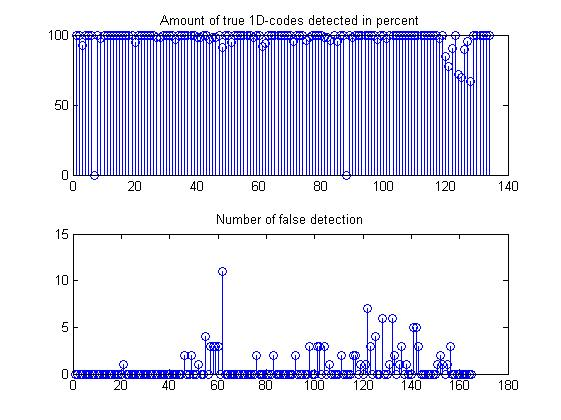
\includegraphics[scale=0.5]{Result24x24_1D}
	\caption{Result for 1D-codes from evaluation of cascade using tile size 24x24, down sampling 2, and no overlap}
	\label{Result24x24_1D}
\end{figure}

\begin{figure}[H]
\centering
	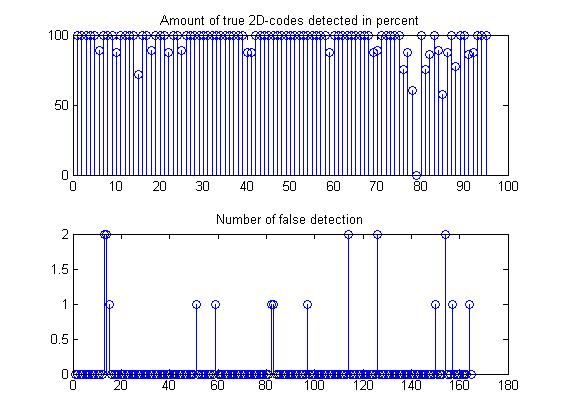
\includegraphics[scale=0.5]{Result24x24_2D}
	\caption{Result for 2D-codes from evaluation of cascade using tile size 24x24, down sampling 2, and no overlap}
	\label{Result24x24_2D}
\end{figure}

\begin{figure}[H]
\centering
	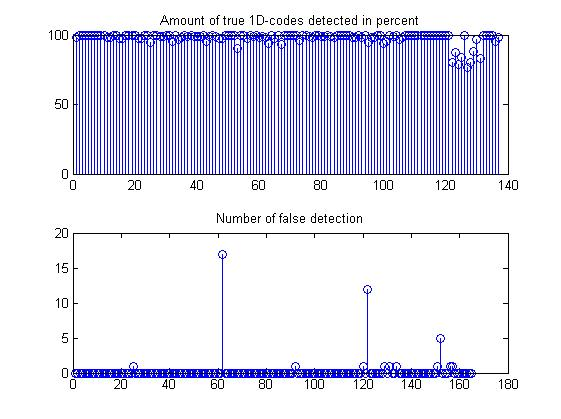
\includegraphics[scale=0.5]{Result32x32_1D}
	\caption{Result for 1D-codes from evaluation of cascade using tile size 32x32, down sampling 2, and overlap 2}
	\label{Result32x32_1D}
\end{figure}

\begin{figure}[H]
\centering
	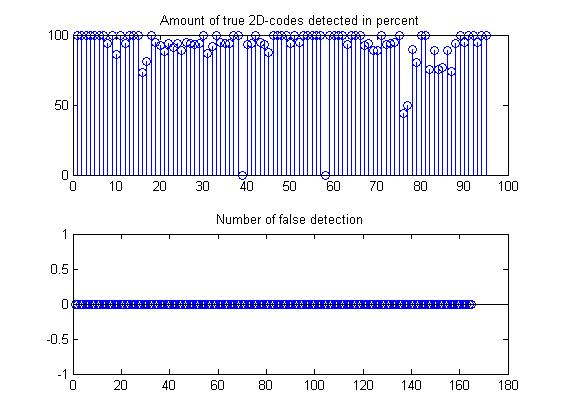
\includegraphics[scale=0.5]{Result32x32_2D}
	\caption{Result for 2D-codes from evaluation of cascade using tile size 24x24, down sampling 2, and no overlap}
	\label{Result24x24_2D}
\end{figure}

\begin{figure}[H]
\centering
	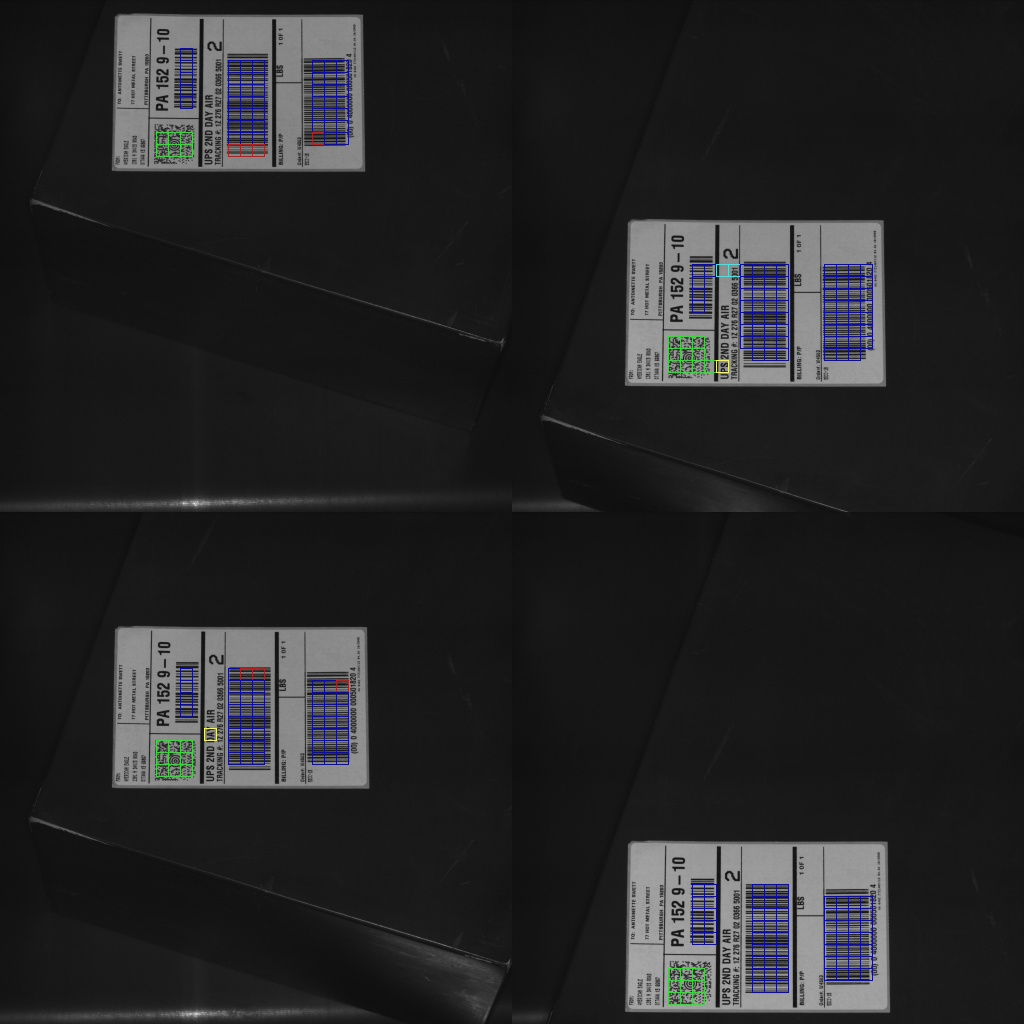
\includegraphics[scale=0.25]{Result24x24}
	\caption{Result from evaluation of cascade using tile size 32x32, down sampling 2, and overlap 2}
	\label{Result32x32}
\end{figure}

\section{Conclusions}
\label{sec:Conclusions}
The two variants of the cascade gave rather similar results. Both the structure tensor and the FAST corner detection are rather good at distinguish between 1D- and 2D-codes.

The first two cases (the two first rows in table 7.11 and table 7.12) gives overall better result, especially regarding the speed. Which one of them that is best depend depend of what is required of the system, regarding speed and accuracy.

One alternative is to omit the distance map feature in the cascade and only use standard deviation and structure tensor for detection of 1D-codes. The result is still rather good, the amount of true detections is even higher but the amount of false tiles will increase.

The amount of true tiles detected can in some cases seem a bit weak, especially for 2D-codes. In the upper graph in \ref{Result24x24_2D} one can see that in one image there are no detections at all. This is the case when the codes are at the border of the image and only a small part are inside. Since in this case only a few tiles will cover the codes there is a big chance that these will be lost in the post-processing. The alternative is to reduce the amount of post-processing but this will instead lead to more false tiles.  

% Local Variables:
% TeX-master: "main.tex"
% End:

\chapter{Further investigations}
\label{sec:Further investigations}
There are a lot of different 2D-codes that are currently used. The system has so far only been tested on Maxicodes. Since other kinds of 2D-codes have similar structure they will presumably give a very similar result. Maxicodes should be more difficult to detect then most other types of 2D-codes since it consists of small circular areas. Most other types of 2D-codes, e.g. QR-codes consists instead of small squares, this should make them even more distinguishable then Maxicodes.

The system could also be tested on a more complicated data set. If one would use a data set that contains more details in the background the system would probably detect a lot more false tiles. However many of the data sets that are available look very similar to the one that has been used.

To speed up the system even further one possibility could be to train a cascade for the local binary pattern alone. Since the LBP has 256 features it is likely that some of these features are more common than others for 2D-codes. If the system is trained to use these features in a certain order it would probably speed up the system. However since the LBP features have been used in the last step of the cascade and the amount of data already has been reduced a lot it is uncertain if this will make much impact.

Postprocessing 



\backmatter

%\bibliography{IEEEfull,myrefs}
\bibliography{References}
\printindex

\end{document}
